\documentclass[a4paper,11pt]{article}
\usepackage[left=2.5cm, right=2.5cm, top=1.5cm, bottom=1.5cm]{geometry}
\usepackage{graphicx}
\usepackage{amssymb}
\usepackage{amsmath}
\usepackage{xcolor}
\usepackage[active,tightpage]{preview}
\usepackage{hyperref}
\usepackage{pythonhighlight}

\hypersetup{ %color attributes of citation, link, etc.
    colorlinks=true,
    linkcolor=blue,
    filecolor=gray,
    urlcolor=blue,
    citecolor=blue,
}

\setlength{\parindent}{0pt}

\renewcommand{\PreviewBorder}{1in}
\newcommand{\Newpage}{\end{preview}\begin{preview}}
\newcommand{\matlab}{\textsc{Matlab}} %very important and totally necessary addition
\newcommand{\parallelsum}{\mathbin{\!/\mkern-5mu/\!}}

\newcommand\Item[1][]{%
  \ifx\relax#1\relax  \item \else \item[#1] \fi
  \abovedisplayskip=0pt\abovedisplayshortskip=0pt~\vspace*{-\baselineskip}}

%'codify' text for snippets
\usepackage{xcolor}
\definecolor{codegray}{gray}{1}
\newcommand{\code}[1]{\colorbox{codegray}{\texttt{#1}}}


\graphicspath{ {../images/} }
           
\begin{document}
\begin{preview}
\title{\LARGE{\textbf{ECEN405 Lab 4 Report\\Boost Converter}}}
\author{Niels Clayton : 300437590\\\textbf{Lab Partner:} Nickolai Wolfe}
\date{}
\maketitle
\hrule

\section{Boost Converter Calculations}

Calculate output voltage $V_{out}$ for:\\
$V_{in} = 20V$\\
$D = o.333$

\begin{align*}
  V_{out}&=\frac{1}{1-D}V_{in}\\\\
  &=\frac{1}{1-0.333}20\\
  &= 30V\\\\
\end{align*}

Calculate the output current $I_{out}$ for:\\
$R_L=500\Omega$

\begin{align*}
  I_{out}&=\frac{V_{out}}{R_{L}}\\\\
  &=\frac{30}{500}\\
  &= 0.06A\\\\
\end{align*}

Calculate the inductor current ripple $I_{\Delta}$ for:\\
$I_{ripple} = 20\%$

\begin{align*}
  I_{delta}&=I_{ripple}\cdot I_{out}\cdot\frac{V_{out}}{V_{in}}\\\\
  &=0.2\cdot 0.06\cdot\frac{30}{20}\\
  &= 0.018A
\end{align*}

Calculate the switching frequency $f_s$ for:\\
$L =4mH$

\begin{align*}
  f_{s}&=\frac{V_{in}\left(V_{out}-V_{in}\right)}{L\cdot I_{\Delta}\cdot V_{out}}\\\\
  &=\frac{20\left(30-20\right)}{0.004\cdot 0.018\cdot 30}\\
  &= 92,592Hz\\\\
\end{align*}

Calculate the output voltage ripple $V_{\Delta}$:

\begin{align*}
  I_{outmax}&=I_{out}+\left(\frac{I_{\Delta}}{2}\right)\\\\
  &=0.06+\left(\frac{0.018}{2}\right)\\
  &=0.069\\\\
  V_{\Delta} &= \frac{I_{outmax}\cdot D}{f_{s}\cdot C}\\\\
  &= \frac{0.069\cdot 0.333}{92592\cdot 100\mu}\\
  &=0.002484
\end{align*}


\section{Low Side MOSFET Drain Voltage}

\begin{center}
  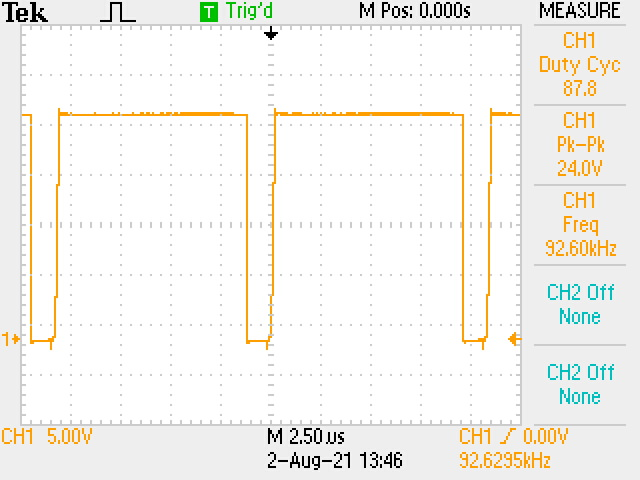
\includegraphics[width = 0.8\textwidth]{drain_voltage.jpg}

  \textit{Low Side MOSFET Drain Voltage From Oscilloscope with a 10\% duty cycle}
\end{center}

From the image above we can see that the voltage at the drain of the low side MOSFET has been scaled to be larger than the 5V control signal. We can also see that the 10\% duty cycle has been inverted, giving a 90\% duty cycle. This is due to the MOSFET pulling the voltage at the drain to ground when switched on. 

We are also able to see that there is very little ringing on the output signal, with very little over and undershoot. 

Finally it can be seen that the falling edge of the voltage waveform is very sharp, however the rising edge as a slight slope to it, this is most likely due to us visualising the charging curve of the capacitor.


\section{Boost Converter Efficiency vs Output Current}

\begin{center}
  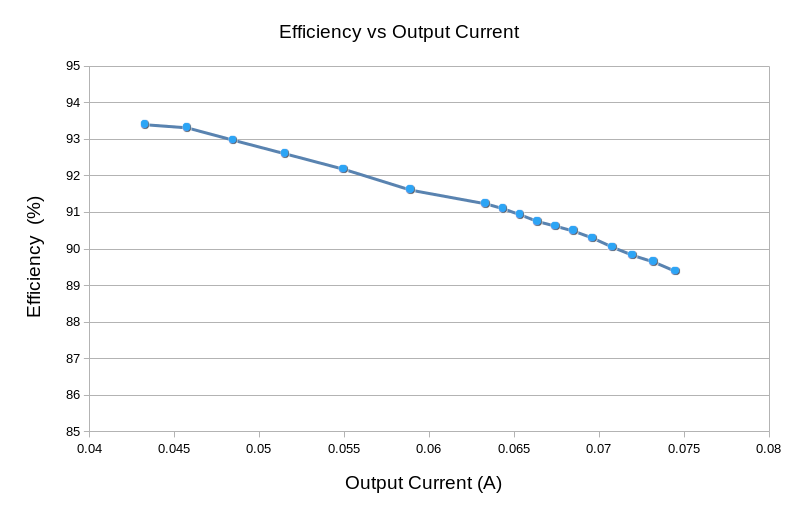
\includegraphics[width = 0.8\textwidth]{Efficiency.png}

  \textit{Boost Converter Efficiency Plot}
\end{center}

In the image above we can see the efficiency vs output current plot of the boost converter built in the lab. We can see from this plot that this seems to be a linear relationship across the output current range we tested. We can also clearly see that as the output current increases, the efficiency of the converter will decrease.


\end{preview}
\end{document}